% generated by scripts/thesis_figures.py (coolant); do not edit by hand
\definecolor{figblue}{HTML}{2A78D6}\definecolor{figorange}{HTML}{EB6834}%
\definecolor{figgreen}{HTML}{1BAF7A}\definecolor{figgrey}{HTML}{898781}%
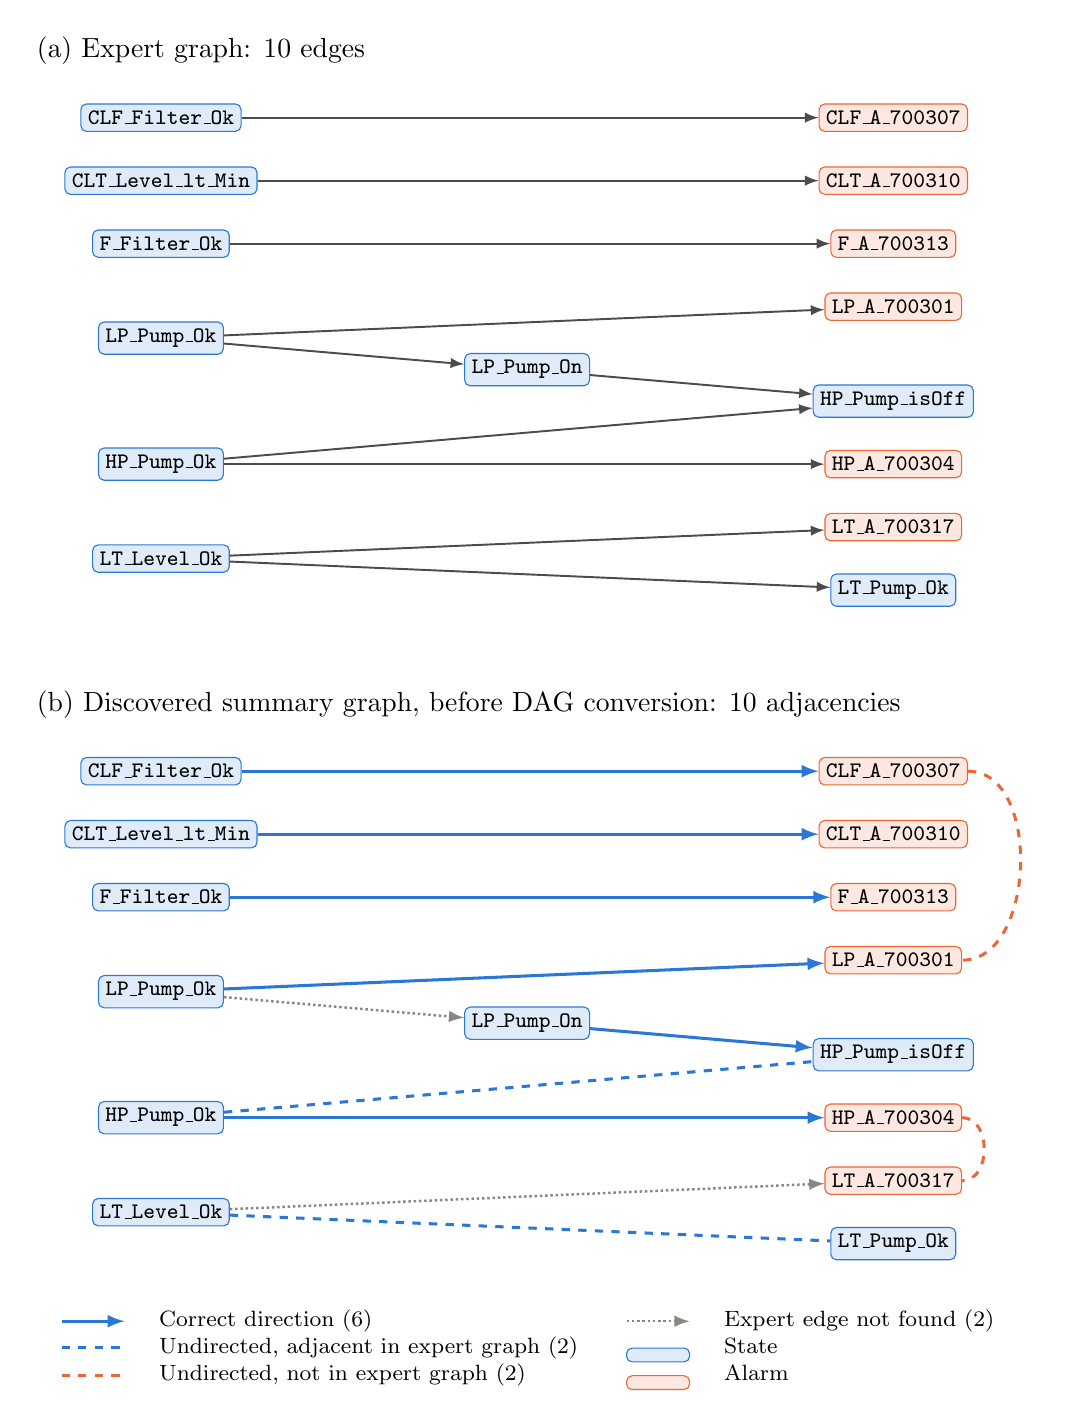
\begin{tikzpicture}[>=latex,
  st/.style={draw=figblue, fill=figblue!15, rounded corners=2pt, inner sep=2.5pt, font=\footnotesize\ttfamily},
  al/.style={draw=figorange, fill=figorange!15, rounded corners=2pt, inner sep=2.5pt, font=\footnotesize\ttfamily}]
\node[anchor=south west, font=\normalsize] at (-1.7, 0.55) {(a) Expert graph: 10 edges};
\node[st] (a-CLF-Filter-Ok) at (0, 0.00) {CLF\_Filter\_Ok};
\node[al] (a-CLF-A-700307) at (9.3, 0.00) {CLF\_A\_700307};
\node[st] (a-CLT-Level-lt-Min) at (0, -0.80) {CLT\_Level\_lt\_Min};
\node[al] (a-CLT-A-700310) at (9.3, -0.80) {CLT\_A\_700310};
\node[st] (a-F-Filter-Ok) at (0, -1.60) {F\_Filter\_Ok};
\node[al] (a-F-A-700313) at (9.3, -1.60) {F\_A\_700313};
\node[st] (a-LP-Pump-Ok) at (0, -2.80) {LP\_Pump\_Ok};
\node[al] (a-LP-A-700301) at (9.3, -2.40) {LP\_A\_700301};
\node[st] (a-LP-Pump-On) at (4.65, -3.20) {LP\_Pump\_On};
\node[st] (a-HP-Pump-isOff) at (9.3, -3.60) {HP\_Pump\_isOff};
\node[st] (a-HP-Pump-Ok) at (0, -4.40) {HP\_Pump\_Ok};
\node[al] (a-HP-A-700304) at (9.3, -4.40) {HP\_A\_700304};
\node[st] (a-LT-Level-Ok) at (0, -5.60) {LT\_Level\_Ok};
\node[al] (a-LT-A-700317) at (9.3, -5.20) {LT\_A\_700317};
\node[st] (a-LT-Pump-Ok) at (9.3, -6.00) {LT\_Pump\_Ok};
\draw[->, draw=black!70, line width=0.7pt] (a-CLF-Filter-Ok) -- (a-CLF-A-700307);
\draw[->, draw=black!70, line width=0.7pt] (a-F-Filter-Ok) -- (a-F-A-700313);
\draw[->, draw=black!70, line width=0.7pt] (a-HP-Pump-Ok) -- (a-HP-A-700304);
\draw[->, draw=black!70, line width=0.7pt] (a-HP-Pump-Ok) -- (a-HP-Pump-isOff);
\draw[->, draw=black!70, line width=0.7pt] (a-LT-Level-Ok) -- (a-LT-A-700317);
\draw[->, draw=black!70, line width=0.7pt] (a-LT-Level-Ok) -- (a-LT-Pump-Ok);
\draw[->, draw=black!70, line width=0.7pt] (a-LP-Pump-Ok) -- (a-LP-A-700301);
\draw[->, draw=black!70, line width=0.7pt] (a-LP-Pump-Ok) -- (a-LP-Pump-On);
\draw[->, draw=black!70, line width=0.7pt] (a-LP-Pump-On) -- (a-HP-Pump-isOff);
\draw[->, draw=black!70, line width=0.7pt] (a-CLT-Level-lt-Min) -- (a-CLT-A-700310);
\node[anchor=south west, font=\normalsize] at (-1.7, -7.75) {(b) Discovered summary graph, before DAG conversion: 10 adjacencies};
\node[st] (b-CLF-Filter-Ok) at (0, -8.30) {CLF\_Filter\_Ok};
\node[al] (b-CLF-A-700307) at (9.3, -8.30) {CLF\_A\_700307};
\node[st] (b-CLT-Level-lt-Min) at (0, -9.10) {CLT\_Level\_lt\_Min};
\node[al] (b-CLT-A-700310) at (9.3, -9.10) {CLT\_A\_700310};
\node[st] (b-F-Filter-Ok) at (0, -9.90) {F\_Filter\_Ok};
\node[al] (b-F-A-700313) at (9.3, -9.90) {F\_A\_700313};
\node[st] (b-LP-Pump-Ok) at (0, -11.10) {LP\_Pump\_Ok};
\node[al] (b-LP-A-700301) at (9.3, -10.70) {LP\_A\_700301};
\node[st] (b-LP-Pump-On) at (4.65, -11.50) {LP\_Pump\_On};
\node[st] (b-HP-Pump-isOff) at (9.3, -11.90) {HP\_Pump\_isOff};
\node[st] (b-HP-Pump-Ok) at (0, -12.70) {HP\_Pump\_Ok};
\node[al] (b-HP-A-700304) at (9.3, -12.70) {HP\_A\_700304};
\node[st] (b-LT-Level-Ok) at (0, -13.90) {LT\_Level\_Ok};
\node[al] (b-LT-A-700317) at (9.3, -13.50) {LT\_A\_700317};
\node[st] (b-LT-Pump-Ok) at (9.3, -14.30) {LT\_Pump\_Ok};
\draw[draw=figorange, line width=1.1pt, dashed] (b-CLF-A-700307.east) to[out=0, in=0, looseness=1] (b-LP-A-700301.east);
\draw[->, draw=figblue, line width=1.1pt] (b-CLF-Filter-Ok) -- (b-CLF-A-700307);
\draw[->, draw=figblue, line width=1.1pt] (b-CLT-Level-lt-Min) -- (b-CLT-A-700310);
\draw[->, draw=figblue, line width=1.1pt] (b-F-Filter-Ok) -- (b-F-A-700313);
\draw[draw=figorange, line width=1.1pt, dashed] (b-HP-A-700304.east) to[out=0, in=0, looseness=1.2] (b-LT-A-700317.east);
\draw[->, draw=figblue, line width=1.1pt] (b-HP-Pump-Ok) -- (b-HP-A-700304);
\draw[draw=figblue, line width=1.1pt, dashed] (b-HP-Pump-Ok) -- (b-HP-Pump-isOff);
\draw[->, draw=figblue, line width=1.1pt] (b-LP-Pump-Ok) -- (b-LP-A-700301);
\draw[->, draw=figblue, line width=1.1pt] (b-LP-Pump-On) -- (b-HP-Pump-isOff);
\draw[draw=figblue, line width=1.1pt, dashed] (b-LT-Level-Ok) -- (b-LT-Pump-Ok);
\draw[->, draw=figgrey, line width=0.9pt, densely dotted] (b-LT-Level-Ok) -- (b-LT-A-700317);
\draw[->, draw=figgrey, line width=0.9pt, densely dotted] (b-LP-Pump-Ok) -- (b-LP-Pump-On);
\node[anchor=north, font=\footnotesize] at (4.65, -15.00) {\begin{tabular}{@{}cl@{\hspace{6mm}}cl@{}}
\tikz[baseline=-0.6ex]\draw[->, draw=figblue, line width=1.1pt] (0,0) -- (0.8,0); & Correct direction (6) & \tikz[baseline=-0.6ex]\draw[->, draw=figgrey, line width=0.9pt, densely dotted] (0,0) -- (0.8,0); & Expert edge not found (2) \\
\tikz[baseline=-0.6ex]\draw[draw=figblue, line width=1.1pt, dashed] (0,0) -- (0.8,0); & Undirected, adjacent in expert graph (2) & \tikz[baseline=-0.6ex]\node[st, minimum width=8mm] {};& State \\
\tikz[baseline=-0.6ex]\draw[draw=figorange, line width=1.1pt, dashed] (0,0) -- (0.8,0); & Undirected, not in expert graph (2) & \tikz[baseline=-0.6ex]\node[al, minimum width=8mm] {};& Alarm \\
\end{tabular}};
\end{tikzpicture}
